%$SI_AUX$%
\documentclass[%
aip,
% jmp,
% bmf,
% sd,
% rsi,
amsmath,amssymb,
%preprint,%
reprint,%
%author-year,%
%author-numerical,%
% Conference Proceedings
]{revtex4-2}

\usepackage{graphicx}% Include figure files
\usepackage{dcolumn}% Align table columns on decimal point
\usepackage{bm}% bold math
%\usepackage[mathlines]{lineno}% Enable numbering of text and display math
%\linenumbers\relax % Commence numbering lines

%\usepackage[utf8]{inputenc}
\usepackage[T1]{fontenc}
\usepackage{mathptmx}

\usepackage{amsmath}
%\usepackage{refcheck}
\usepackage{graphicx}% Include figure files
\usepackage{dcolumn}% Align table columns on decimal point
\usepackage{bm}% bold math
\usepackage{hyperref}% add hypertext capabilities
%\usepackage[mathlines]{lineno}% Enable numbering of text and display math
%\linenumbers\relax % Commence numbering lines
\usepackage[capitalize]{cleveref}
\newcommand{\rhoN}{\ensuremath{\rho_{\rm N}}}
\newcommand{\kB}{\ensuremath{k_{\rm B}}}

\newcommand{\abinitio}{ab initio}
\newcommand{\HS}{\ensuremath{\rm HS}}
\newcommand{\IPL}{\ensuremath{\rm IPL}}
\newcommand{\LJ}{\ensuremath{\rm LJ}}
\newcommand{\EXP}{\ensuremath{\rm EXP}}
\newcommand{\Hefour}{\ensuremath{^4\mathrm{He}}}
\newcommand{\frakB}{\ensuremath{\mathfrak{B}}}
\newcommand{\sr}{\ensuremath{s^{\rm{r}}}}
\newcommand{\splus}{\ensuremath{s^+}}
\newcommand{\cvr}{\ensuremath{c_v^{\rm{r}}}}
\newcommand{\myA}{\ensuremath{\widetilde A}}
\newcommand{\myAr}{\ensuremath{\widetilde A^{\rm r}}}
\newcommand{\neff}{\ensuremath{n_{\rm eff}}}
\newcommand{\myAo}{\ensuremath{\widetilde A^{0}}}
\newcommand{\nsrR}{\ensuremath{-s^{\rm{r}}/\kB}}
\newcommand{\etazero}{\ensuremath{\eta_{\rhoN\to 0}}}
\newcommand{\noi}{\noindent}
\newcommand{\Batt}{\ensuremath{B_{2,\rm att}}}
\newcommand{\Brep}{\ensuremath{B_{2,\rm rep}}}
\newcommand{\Arrhenius}{``Arrhenius"}
\newcommand{\lambdazero}{\ensuremath{\lambda_{\rhoN\to 0}}}
\newcommand{\Dzero}{\ensuremath{D_{\rhoN\to 0}}}
\newcommand{\ar}{\ensuremath{a^{\rm{r}}}}
\newcommand{\alphar}{\ensuremath{\alpha^{\rm{r}}}}
\newcommand{\deriv}[3]{\ensuremath{  \left(\dfrac{\partial #1}{\partial #2}\right)_{#3} }}
\newcommand{\rmderiv}[2]{\ensuremath{ \dfrac{{\rm d} #1}{{\rm d} #2} }}
\newcommand{\rmd}{\ensuremath{ {\rm d} }}

\newcommand{\copyrightfootnote}{\thanks{Contribution of the National Institute of Standards and Technology, not subject to copyright in the US}}

\usepackage{xcolor}
\usepackage{soul}

\newcommand{\TODO}[1]{{\color{red} XXX #1 XXX \message{LaTeX Warning: TODO: #1}}}

\newcommand{\question}[1]{%
    \colorlet{foo}{yellow}%
    \sethlcolor{foo}\hl{#1} \message{TODO: #1}}%

\newcommand{\papertitle}{A super awesome paper title {\copyrightfootnote}}

\newcommand{\abstracttext}{This paper develops a revolutionary novel understanding of physics.}
\usepackage{cancel}
\usepackage{xcolor}
\usepackage{float}
%\usepackage{natbib}
%\bibliographystyle{unsrt}

\usepackage{zref-xr,zref-user}
\zxrsetup{verbose}
\zexternaldocument*{SI_paper}	

\graphicspath{{figs/}}

\begin{document}
	
%\usepackage[showframe,%Uncomment any one of the following lines to test 
%%scale=0.7, marginratio={1:1, 2:3}, ignoreall,% default settings
%%text={7in,10in},centering,
%%margin=1.5in,
%%total={6.5in,8.75in}, top=1.2in, left=0.9in, includefoot,
%%height=10in,a5paper,hmargin={3cm,0.8in},
%]{geometry}

%\preprint{APS/123-QED}
%
\title{\papertitle}% Force line breaks with \\
%%\thanks{A footnote to the article title}%
%
\author{Ian H. Bell}
\email{ian.bell@nist.gov}
%\thanks{Corresponding author}
% \altaffiliation[Also at ]{Physics Department, XYZ University.}%Lines break automatically or can be forced with \\
 \affiliation{%
Applied Chemicals and Materials Division, National Institute of Standards and Technology, Boulder, CO 80305
 }

\date{\today}% It is always \today, today,
             %  but any date may be explicitly specified

\begin{abstract}
\abstracttext
%\begin{description}
%\item[Usage]
%Secondary publications and information retrieval purposes.
%\item[Structure]
%You may use the \texttt{description} environment to structure your abstract;
%use the optional argument of the \verb+\item+ command to give the category of each item. 
%\end{description}
\end{abstract}

%\keywords{Suggested keywords}%Use showkeys class option if keyword
                              %display desired
\maketitle
%\tableofcontents

    
    \section{Introduction}

    Some folks wrote some stuff \cite{Span-BOOK-2000}

    See the very warm figure: \cref{fig:hot}.
    See the very cool figure: \cref{fig:cold}.
    
    See the Section \zref{sec:CIneff} in the supporting information

    \begin{figure}[H]
    \caption{Hot! \label{fig:hot}}
    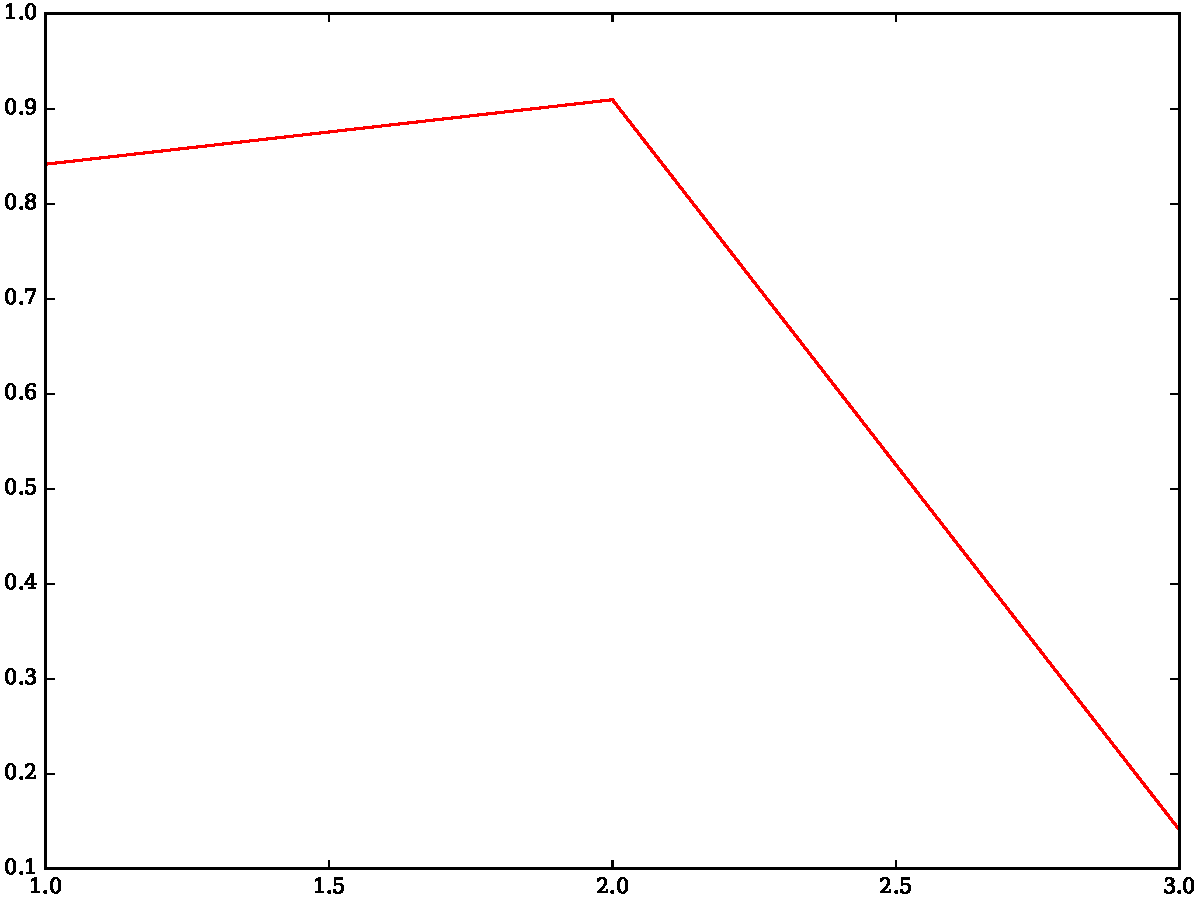
\includegraphics[width=3in]{hot}
    \end{figure}

    \begin{figure}[H]
    \caption{Cold! \label{fig:cold}}
    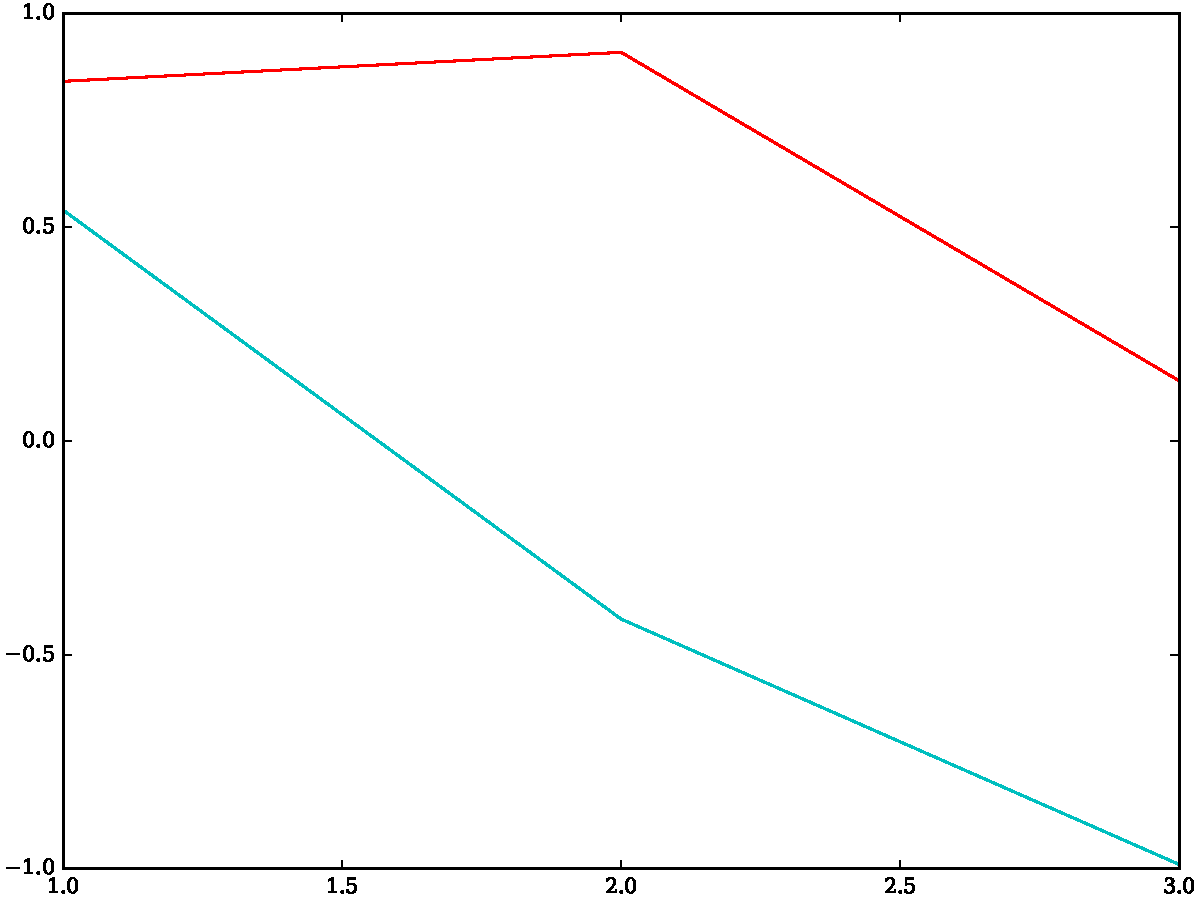
\includegraphics{cold}
    \end{figure}
    
%    \begin{tocentry}
%    \begin{center}
%    \includegraphics[height=1.75in]{TOC_image}
%    \end{center}
%    \end{tocentry}

    \section{Supplementary Material}
    In order to ensure reproducibility of our results, the supplementary material includes:
    \begin{itemize}
    	\item The Python code and analysis for ....
    \end{itemize}

    \begin{acknowledgments}
    NIST folks
    \end{acknowledgments}
    
	\bibliography{CoolPropBibTeXLibrary}
\end{document}